\documentclass{article}
\usepackage[utf8]{inputenc}

% \title{Group of Seven Report}
% \author{1756850 Alkhamra, Othman Bader \\
% 1739256 Benicek, David \\
% 1770922 Bari, Aadam Ali \\
% 1425704 Mankani Vinod, Hitesh \\
% 1755013 Obimma, Timothy Uzochukwu \\ 
% 1783087 Vaddiraju, Nagarjuna}
% \date{January 2018}

\usepackage{natbib}
\usepackage{graphicx}
\usepackage{url}

\begin{document}
	
	\begin{titlepage}
		\newcommand{\HRule}{\rule{\linewidth}{0.5mm}} % Defines a new command for horizontal lines, change thickness here
		\newcommand{\hRule}{\rule{\linewidth}{0.1mm}} % Defines a new command for horizontal lines, change thickness here
		\centering
		
\includegraphics[width=0.2\textwidth]{kcl.png}\par\vspace{1cm}
		\textsc{\LARGE King's College London}\\[1.5cm] % Main heading such as the name of your university/college
		\textsc{\large 7CCSMGPR}\\[0.5cm] % Major heading such as course name
		\textsc{\Large Group Project}\\[0.5cm] % Minor heading such as course title
		\HRule\\[0.4cm]
		{\huge\bfseries Group of Seven Report}\\[0.4cm] % Title of your document
		\HRule\\[1.5cm]
		\vspace{1cm}
		\textit{Authors: }\vspace{0.5cm}
		\begin{center}
			\begin{tabular}{ c|c|c } 
				\hline
				\textbf{Number} & \textbf{Name} & \textbf{Email} \\
				\hline
				1756850 & Othman \textsc{Alkhamra} &  othman.alkhamra@kcl.ac.uk \\ 
				\hline
				1739256 & David \textsc{Benicek} &  david.benicek@kcl.ac.uk \\ 
				\hline
				1770922 & Aadam \textsc{Bari} &  
				aadam.bari@kcl.ac.uk\\ 
				\hline
				1425704 & Hitesh \textsc{Mankani Vinod} &  hitesh.mankani\_vinod@kcl.ac.uk \\ 
				\hline
				1755013 & Timothy \textsc{Obimma} &  timothy.obimma@kcl.ac.uk \\ 
				\hline
				1783087 & Nagarjuna \textsc{Vaddiraju} &  nagarjuna.vaddiraju@kcl.ac.uk \\ 
				
				\hline
			\end{tabular}
		\end{center}
		
		\vfill
		supervised by\par
		Dr.~Laurence \textsc{Tratt}\\
		\vfill
		{\large \today\par}
	\end{titlepage}
	% \maketitle
	\newpage
	\pagenumbering{roman}
	\tableofcontents
	\newpage
	\pagenumbering{arabic}
	\section{Introduction}
	In real life, we have different objects such as spheres, cubes ... etc. What's mutual between them is that they are all geometry objects. However, those objects might appear in different ways, based on their environment. For example, a glass sphere placed in an environment with many light sources will react in a different way than a metal sphere. And so, it is clear that different factors such as the material type, light sources and many other factors, will produce many different outputs. \\
	\par Ray tracing is one of those techniques which helps in producing different images for different environment variables. It is widely used in producing films, video games, animations and many other areas. It can be applied on any object and not just geometry objects.
	\subsection{What is the Idea behind  Ray Tracing?}
	Before discussing the idea behind ray tracing, and explaining its algorithm. Let's begin with listing the basic required elements to run the ray tracing algorithm. Those elements will be in one container which will be called \textbf{scene}. The elements of the scene are:
	\begin{itemize}
		\item \textbf{Object(s)}: a scene can contain one or many objects. Each object can be one of the previously mentioned objects or any other object, which exists in real life. For example, an object could be a sphere, triangle, tree, car, building ... etc.
		\item \textbf{Light source(s)}: The algorithm of ray tracing itself doesn't require having a light source. However, a scene without any light source, won't make the use of ray tracing effective.
		\item \textbf{Image Plane}: which is called \textbf{window frame} in our implementation. This plane will have some width and height, and it will be divided into small squares, and each square will be covering a number of pixels on the objects of the scene.
		\item \textbf{Eye or Camera:} In order to render the scene, it is mandatory to have an eye or camera, with some position and some direction, to detect the way of looking to the scene elements. From that eye or camera, rays will be produced, and will go through the image plane.
	\end{itemize}
	\begin{figure}[ht!]
		\centering
		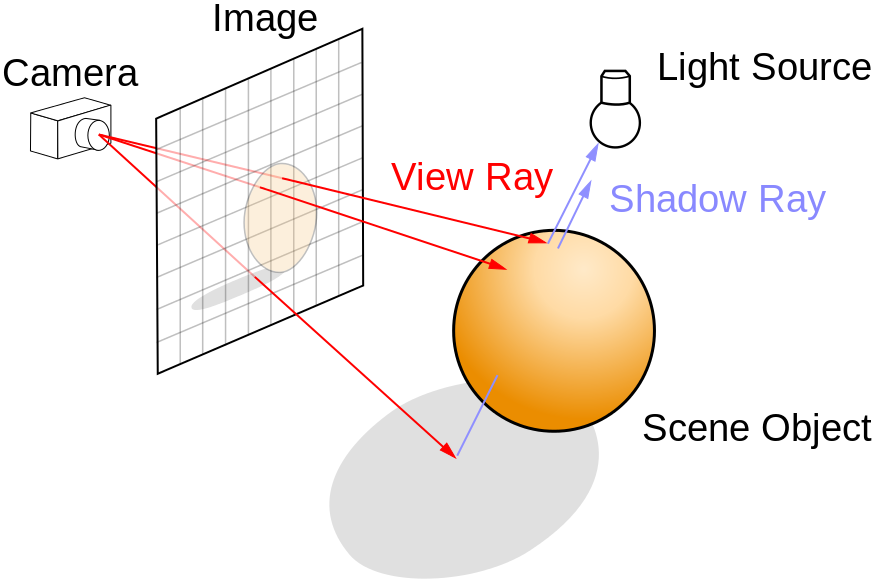
\includegraphics[scale=0.30]{./raytracing.png}
		\caption{Ray Tracing's Scene Elements \cite{raytracingpic}}
		\label{fig:raytracing}
	\end{figure}
	\par \textbf{Figure \ref{fig:raytracing}} shows an example of a scene with the previously listed elements. Now, and after discussing the elements of the scene, it is the time to describe the algorithm of ray tracing. The idea is so simple, in each scene there will an eye or camera, from that camera many rays will be produced and go across the small squares in the image plane, for each ray we need to check whether it intersects with any of the objects or not, and return the colour of that pixel.\\
	\par The algorithm itself is really simple. Nevertheless, it is previously mentioned that environment variables play a big role in the calculations. And so, returning the colour of the pixel, which was hit by the the ray, won't be that simple; since it will require additional computations related to the reflections, shades ... etc. 
	\subsection{Our Solution}
	Although the idea behind ray tracing is simple. But, there are many different problems to be addressed in this program. These problems can be summarised as below:
	\subsubsection{Web Interface}
	In order to define the different elements of the scene, a web interface is developed to allow users enter the different values for the scene elements. Using this interface, the user can add different objects to the scene, with different materials, positions, sizes, colours. Furthermore, adding different lights at different positions with different colours. \\
	\par The challenge here is that objects must be in 3D. And so, we developed a web interface with two options. One option is the 2D option, where the user needs to define an element by providing its values in the top and side views. The other option, is the 3D view, where the user can add elements directly in 3D format.\\
	\par All the functionality in our web interface supports the drag and drop feature. In other words, this means that the user can define the position by clicking on the object, and moving it in any direction.
	\subsubsection{Ray tracing Engine}
	The other part of our system is the back-end engine, where all the calculations are done based on the input received from the web interface. This system was developed using .NET C\#. It includes a post API, which will receive the request from the client, and it is able to render a scene with the followings:
	\begin{itemize}
		\item A scene with the following objects:
		\begin{itemize}
			\item \textbf{Plane}: This object is mainly used to create the walls in the scene. And it has a position, and a normal which decides the orientation, in addition to one of the supported materials.
			\item \textbf{Cube}: Each cube has a size, a position, and one of the supported materials.
			\item \textbf{Sphere}: Each sphere has a radius, centre point, and one of the supported materials.
		\end{itemize}
		The  \textbf{supported materials} are:
		\begin{itemize}
			\item \textbf{Phong materials}:  which follows the phong theory such as chalk, metal, plastic. The difference between those materials is the values of diffusion, specular coefficients and the light colour influence.
			\item \textbf{Flat material}: which is the simplest material, that will return the colour of that object regardless to any other environment variables and parameters.
			\item \textbf {Glass material}: this material is the most complicated one, which will do many different calculations in order to calculate the colour of each pixel of that object.
		\end{itemize}
		Each of these materials can have a colour chosen by the user, or just use the default colour, if \textbf{nothing} is received.
		\item A scene with multiple light sources at different positions and colours.
		\item A scene with perspective camera. Each camera has a position, direction of how to look at the image plane, and distance from that plane.
	\end{itemize}
	\section{Review}
	\section{Requirements and design}
	\section{Implementation}
	\subsection{Front End}
	\subsection{Back-end}
	\subsubsection{Unit Testing}
	
	\section{Team work}
	
	%In this section: Describe how you worked together, including the tools and processes you used to facilitate group work.
	
	\subsection{Process}
	Weekly meetings
	At the start of each meeting standup style sync up:
	Everyone speaks, says what they did, what still needs to be done, calls out any blockers that we can go over in the follow on meeting.
	Discussion: 
	Talk about what the next steps are, what could be improved, what has blocked us in the previous sprint. Try arrive at outcomes - outcomes made into tickets
	Next steps:
	Illicit next steps both from discussion and from product roadmap
	
	
	\subsection{Tools}
	Communication
	Non structured: Whatsapp, Facebook
	Structured: Meetings, Git Issues, Git wiki, Pull requests w/ comments
	
	During development: a lot of pair programming, allowing us to cross pollinate ideas and spread knowledge, break up silos.
	
	%!!!!!!!!!!!!!!!!!!!!!!!!!!!!!!!!!!!!!!!!!!!!!!!!!!!!!!!!!!!!!!!!!!!!
	%!!!!!!TODO: I've got all this shit to refactor and put in here: !!!!
	%!!!!!!!!!!!!!!!!!!!!!!!!!!!!!!!!!!!!!!!!!!!!!!!!!!!!!!!!!!!!!!!!!!!!
	% Communication is one of the most important factors when it comes to working in a software engineering team. For our project we decided to utilise a number of different structured and unstructured communication channels. There are a number of great project management and issue tracking tools such as JIRA, Trac or Trello, however, we decided that given the brevity of our project and the relative low number of backlog items (especially at the start) that it would be best to keep our ticket system as close to the codebase as possible. As a result of this, we decided to make use of the inbuilt GitHub issue tracking system. This system does not provide the same calibre of project management tools as some of the forementioned products, however, it does enough for our purposes. We decided to use the GitHub milestone system as a way of scheduling issues for our sprints and implemented a branch naming convention such that we would refer to the issue we're addressing in the name of the branch - \{issue number\}/\{name of branch\}. This simple mechanism has worked tremendously because it ensures that on one hand all branches are addressing exactly one tasks or feature and on the other hand, that all tasks and features have been recorded in an issue. 
	
	% Not all communication can be done over issue summaries and pull requests and therefore we schedule weekly meetings to go over what has been achieved, what needs to be discussed and what is the plan for the following sprint. One could say that we condensed our daily scrum meeting, sprint planning, backlog refinement and sprint review all into one meeting. This is not the correct way of running an Agile project but given that we are not working  on the project full time and that these meetings were kept as brief as possible, it still sticks to the core values of Agile. During the meetings we would discuss the general trajectory of the project and what we want to accomplish in the next seven days, before breaking off into our sub teams and deciding on the issues needed for the week.
	
	% During the course of the sprints, our communication did not fade. We took inspiration from Extreme Programming and met frequently in our work units to engage in pair programming while working on issues. 
	
	% Lastly, to facilitate the smooth operation of the team we used the lowest friction medium for all of us which was a WhatApp group where we have so far discussed everything from meeting times to specific lines of code in pull request. 
	
	
	\section{Evaluation}
	
	% What worked well 
	% Splitting the work into two teams
	% The two teams knew each other better therefore we were able to work more effectively.
	% Focused on Critical tasks first
	% If the task was Critical like SVG implementation then the whole sub-team worked on it. If it was a small task like fixing a bug or making UI better, the tasks were divided between the sub-team.
	
	% What didn't? 
	% Communication between front and back end - e.g colour issue. Improved on it and made communication better but still lacked a bit between the sub-teams and in the sub-teams.
	
	
	% How did you do relative to your plan?
	% Had weekly tasks - aimed to do them before the next meeting. Gave everyone a week to do it. If they were not completed, then a few more days was given.
	% Internal deadline - pushed by one week
	
	% What changes were the result of improved thinking and what changes were forced upon you?
	% Video call instead of group meeting which led to 2 meetings per week??
	
	% How did your team work together? -Goes in team work right?
	
	% What have we achieved and what could we have done if we have more time?
	% More shapes?
	
	% Mention both strengths and weaknesses!!
	
	\clearpage
	\bibliographystyle{plain}
	\bibliography{references}
\end{document}
